\section{Durchführung}
\label{sec:Durchführung}

Der theoretische Aufbau des Experiments befindet sich in \autoref{fig:2}.
\begin{figure}[H]
    \centering
        \centering
        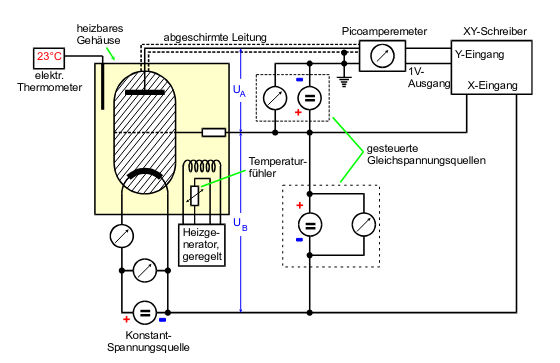
\includegraphics[width=0.7\textwidth]{Bilder/theoaufbau.png}
        \caption{Aufbau des Versuchs (1). \cite{anleitung5}}
    \hfill
    \label{fig:2}
\end{figure}
\noindent Die Installation gemäß des Plans ist in \autoref{fig:3} zu sehen.
\begin{figure}[H]
    \centering
        \centering
        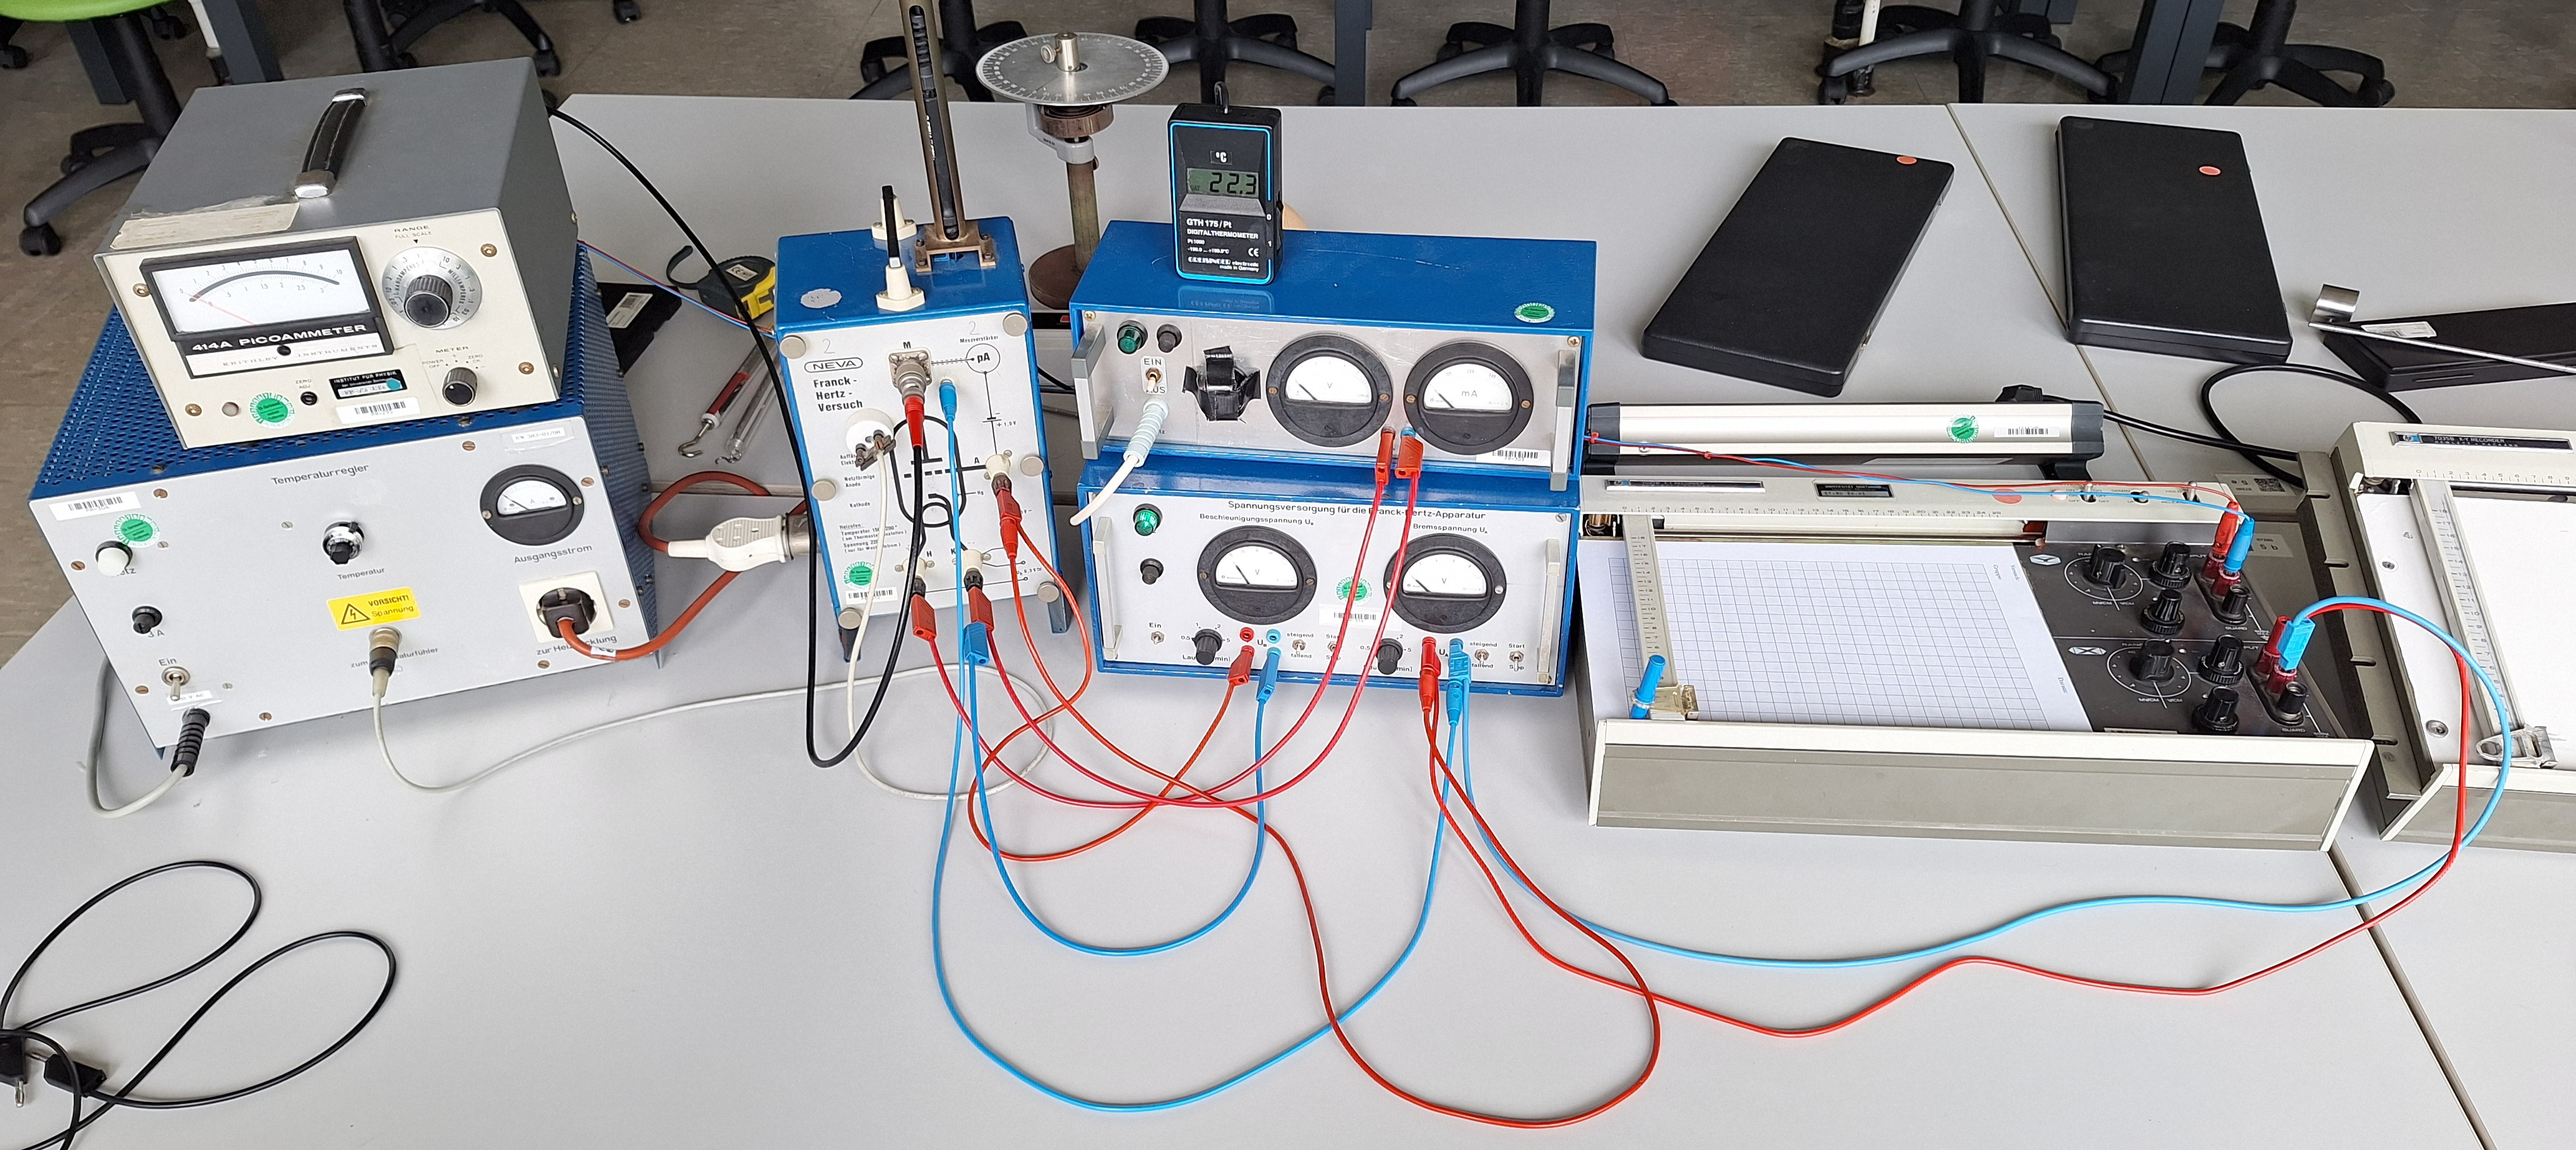
\includegraphics[width=\textwidth]{Bilder/installation.jpg}
        \caption{Aufbau des Versuchs (2).}
    \hfill
    \label{fig:3}
\end{figure}
\noindent Auf der linken Seite ist ein elektronischer Temperaturregler zu 
sehen, welcher die Temperatur des Glaskolbens konstant hält, er liefert Werte 
im Bereich von $373.15 - 473.15 \unit{\kelvin}$. Über dem Regler steht das 
Picoamperemeter. Jenes soll den Auffängerstrom $I_A$ der Anode detektieren.
Rechts dieser Bauten befindet sich das Herzstück des Experiments: Die Franck-
Hertz Röhre mit dem Hg-Dampf, was auf dem Bild nur von der Seite zu sehen ist.
Wiederum rechts der Röhre befindet sich eine Apparatur zur Spannungsregulierung,
sie ist für $U_B$ und $U_A$ zuständig.
\vspace{0.5em}
Für die integrale Energieverteilung der beschleunigten Elektronen wird ersteres 
zunächst auf $U_B = 11 \unit{\volt}$ eingestellt und konstant gelassen. Die
Spannung $U_A$ wird innerhalb einer halben Minute hochgeregelt. Ganz rechts 
liegt der XY-Schreiber, welcher die Stromstärke in Abhängigkeit der Spannung 
aufzeichnet. Dazu wird lediglich ein Blatt Papier in der Vorrichtung befestigt 
und der Schreiber wie gewünscht justiert. Die Messungen für diesen Teil werden 
in einem Bereich von $T = 413.15 - 433.15 \unit{\kelvin}$ durchgeführt.
\vspace{0.5em}
Für den zweiten Teil des Experiments sollen die tatsächlichen Franck-Hertz Kurven 
erstellt werden. Dazu wird für zwei verschiedene Temperaturen jeweils eine Kurve 
mithilfe des XY-Schreibers aufgenommen. Nun wird die Stromstärke $I_A$ in 
Abhängigkeit der Beschleunigungsspannung gemessen. Dazu wird die Bremsspannung 
konstant auf $U_A = 1 \unit{\volt}$ eingestellt und $U_B$ im Bereich von $0 -
60 \unit{\volt}$ hochgestellt.